\section{Crystals}

\paragraph{Crystals}
Solid state physics, as we will study it, is concerned with crystals. A crystal is an arrangement of atoms which is repeated periodically. When developing the physics of crystals, we will assume their repetition to be infinite.

\paragraph{Basis}
The arrangement of atoms which is repeated in a crystal is termed the basis.

\paragraph{Lattices}
The set of points to which the basis is attached is termed the lattice.

\paragraph{Bravais Lattices}
A Bravais lattice is a lattice such that the arrangement of lattice points looks exactly equal from any lattice point. This turns out to be equivalent to the lattice being infinite and symmetric under certain discrete translations. We will treat crystal lattices as Bravais lattices.

The two-dimensional Bravais lattices are the rectangular,

\begin{figure}[!ht]
	\centering
	\subfloat[Square.]
	{
		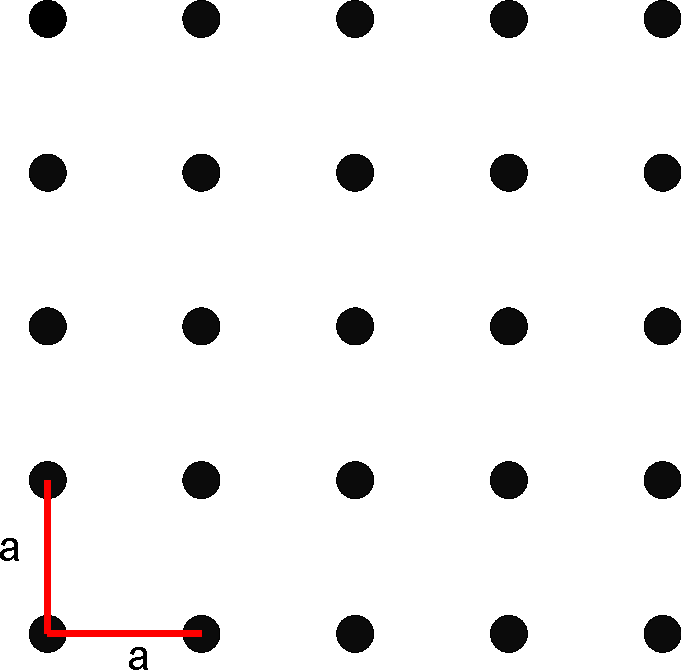
\includegraphics[width = 0.3\textwidth]{./Images/2d_square.pdf}
	}
	\hfil
	\subfloat[Rectangular.]
	{
		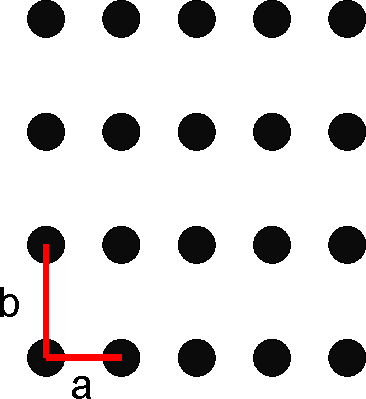
\includegraphics[width = 0.3\textwidth]{./Images/2d_rectangular.pdf}
	}
\end{figure}

%TODO: Add 2D and 3D Bravais lattices

\paragraph{Lattice Vectors}
The set $\{\vb{a}_{i}\}$ of lattice vectors of a Bravais lattice is the smallest possible set of vectors such that translating the lattice by $u_{i}\vb{a}_{i}$, where the $u_{i}$ are integers, leaves the lattice unchanged. There is an infinite number of ways to define the lattice vectors of a given lattice.

\paragraph{Primitive Lattice Vectors}
A set of lattice vectors is primitive if any two equivalent points are connected by integer combinations of the lattice vectors.

\paragraph{Crystal Axes}
The crystal axes are a set of directions that span space. These may be chosen according to, for instance, the primitive lattice vectors or other directions connected to the symmetry of the lattice.

\paragraph{Crystal Cell}
The crystal cell is the repeat unit of the crystal. It may be constructed in an infinite number of ways.

\paragraph{Lattice Constants}
Lattice constants are a set of parameters defining the dimensions of the cell.

\paragraph{Primitive Cell}
The primitive cell is a minimum-volume cell. It contains only one lattice point, and is thus termed a unit cell. Its infinite translation throughout space yields the lattice.

\paragraph{Primitive Basis}
The primitive basis is the basis associated with the primitive cell.

\paragraph{Wigner-Seitz Cell}
The Wigner-Seitz Cell is the cell constructed by for any lattice point dividing space into two at the middle of and normal to the line between the point in question and all other points, and choosing the smallest possible region of space containing the point from this.

\paragraph{Lattice Point Group}
The lattice point group is the group of operations which, applied about a lattice point (i.e. keeping this point fixed), leaves the lattice unchanged. Examples of possible fundamental operations include:
\begin{itemize}
	\item rotations.
	\item reflections.
\end{itemize}

\paragraph{Lattice Space Group}
The space group of the Bravais lattices is the group of symmetries of all Bravais lattices of a given dimensionality. It contains both point groups and translations.

\paragraph{$n$-Fold Rotations}
An $n$-fold rotation is a rotation operation such that it reduces to the identity operation when applied $n$ times. Lattices cannot be symmetric under $5$-fold rotation.

\paragraph{Crystal Planes}
In a cell it is useful to define crystallographic planes. Rather than specifying them in terms of a normal vector, they are specified according to the following rules:
\begin{enumerate}
	\item For each axis, defined by the lattice vectors, identify the intercepts of the plane with the axis.
	\item Compute the reciprocals of each intercept.
	\item Reduce to three integers with the same ratio.
\end{enumerate}
The notation is of the form \cplane{hkl}. A bar above any element indicates that element to be negative. A set of planes equivalent by symmetry may be denoted \cpset{hkl}.

\paragraph{Crystallographic Directions}
Likewise we define crystallographic directions by the notation \cdir{uvw}. The indices are the set of the smallest integers such that they form a vector parallel to the one in question.

\paragraph{Random Stacking}
Randomly stacked crystals are formed by densely packed layers of atoms being stacked without long-range order in the stacking direction.

\paragraph{Polytopism}
Polytopism is a milder variation of random stacking, where the order of the stacked layers is extremely long-range.

%TODO: Add special structures